\author{Andrew Lim}
\title{Predicting film box office openings with Wikipedia}
\date{14 Jan 2013}

\documentclass[10pt]{article}

\usepackage{anysize}
\usepackage[font={small}]{caption}
\usepackage{graphicx}
\usepackage{multicol}
\usepackage{setspace}
\usepackage{url}
\usepackage{wrapfig}

\marginsize{1in}{1in}{1in}{1.25in}
\onehalfspacing

\begin{document}

    \maketitle
    
    \begin{abstract}
        To what extent can Wikipedia be used to measure social interest? In this analysis, I examine the ability of Wikipedia edit data to predict opening box office revenues for US films. I present a simple model fit to films released during 2007-2011 based on features in their Wikipedia articles. While this model's predictive power is probably insufficient for all but the roughest estimates of revenue, it does demonstrate how popular interest in films is reflected in Wikipedia activity. 
    \end{abstract}
    
    \section{Introduction: Wikipedia as a gauge of social interest}
    
    \begin{figure}[ht]
        \centering
        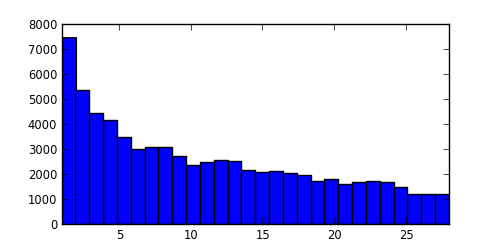
\includegraphics{wikipedia28.png}
        \caption{Count of Wikipedia article edits for the films used in this paper's training dataset over the 4 weeks prior each film's respective release date, bucketed by days before release date that the edits occurred. This graph shows the uptick in editing activity that typically accompanies a film's release.}
        \label{fig:wikipedia-28}
    \end{figure}
    
    \paragraph{}
    According to its article about itself (as of this writing), Wikipedia is ``a collaboratively edited, multilingual, free Internet encyclopedia'' launched in January 2011. \cite{bib:wikipedia} Its articles can be edited by anyone, either anonymously (though the editor's IP address is logged) or with a registered user account. The edit history of each article is saved with a timestamp. Interested users can view any past version of an article, and an article's edit history exhibits an evolving record of Wikipedia's ``knowledge''\footnote{Of course, Wikipedia's highly open policy means both that it contains a stunning breadth of information from contributors with wide-ranging expertise and that said information is sometimes unreliable. For an example that was in the news not long before this paper was written, see \cite{bib:bicholm}, or for Wikipedia's own list of Wikipedia hoaxes, see \cite{bib:wikipedia-hoaxes}.} of its subject. 
    
    \paragraph{}
    As such, Wikipedia's edit history can be viewed as a barometer of social interest. For example, when a person is in the news, edit activity on his or her article often spikes. In fact, Wikipedia has template warnings indicating when an article is likely to be in flux due to a relevant current event. Edit activity on Wikipedia, in this sense, is akin to mentions on social networks like Facebook or Twitter, although perhaps with a smaller participating audience (although many people read Wikipedia, not nearly so many participate in its creation). 
    
    \paragraph{}
    One area where we can try to gauge the degree to which Wikipedia activity reflects social interest is in film box office performance. Films have relatively well-defined release dates prior to which we can measure activity on Wikipedia. They also have well-defined, measurable outcome - revenues at the ticket booth - that is clearly sensitive to popular interest. Theater owners obviously have a direct financial interest in knowing how well a film is going to perform. Advertisers and publicists, sellers of tie-in products, and film journalists have a slightly more indirect but still strong interest; they will want to know how they should spend their time and money. Can we use Wikipedia to usefully predict films' opening box office performances? 
    
    \section{Formulation of problem and data sources}
    
    \paragraph{}
    The specific question I set out to answer was: how accurately, using Wikipedia's help, can we predict the domestic per-theater box office gross of a film released widely in the US, over the first three days\footnote{Films traditionally open on Friday, and their ``opening'' often refers to their gross over the first Friday, Saturday, and Sunday that they are playing. However there are plenty of non-Friday openings as well. Consequently, I've stated the problem in terms of the first three days' worth of grosses.} of its release? 
    
    \paragraph{}
    The data sources I used to answer this question were: 
    
    \begin{itemize}
        \item Box Office Mojo (\url{http://www.boxofficemojo.com/}) - contains detailed box office data. I used it to select the universe of films to analyze and as my source for theatrical release dates, number of opening theaters, and revenues. There is no API - I scraped the data with the Python package \textsf{Beautiful Soup}. 
        \item Rotten Tomatoes (\url{http://www.rottentomatoes.com/}) - a popular movie review aggregator. I used it to obtain descriptive information about films: genres, runtime, MPAA rating, cast and directors, and so on. It offers an API if you register for a key (which is free as of the present writing). 
        \item Wikipedia (English-language) (\url{http://en.wikipedia.org/}) - MediaWiki, the name of the web application upon which Wikipedia is based, offers an API, no registration or key necessary. 
    \end{itemize}
    
    \paragraph{}
    Much of the work involved in data retrieval and formatting was to ensure that data retrieved from these three sources corresponded to the same film; data from Rotten Tomatoes and Wikipedia was obtained by using their APIs' search functionalities, which can lead to incorrect hits if you are not careful. For example, we want to make sure that Rotten Tomatoes data for the 2012 film ``The Lucky One'' is not mapped to the 2008 film ``The Lucky Ones,'' or that for the 2010 film ``Salt'' we do not examine the Wikipedia article for salt, the mineral.\footnote{Box Office Mojo data had to be scraped from HTML, but the HTML was regular and consistent. Rotten Tomatoes has a nice JSON-based API for data retrieval, but its ranking of returns is quirky, sometimes retrieving obscure films or films with similar names (example: Oliver Stone's 2008 biopic ``W.'' was unfindable through search query, even through the website's front end; I had to go to Stone's Rotten Tomatoes page just to find the relevant web page). Wikipedia both has a nice API and solid/consistent lookup, which is all the more impressive given that it contains articles on anything, not just films.} 
    
    \paragraph{}
    The universe of films that I considered were those listed on Box Office Mojo as having opened in at least 1000 theaters. I manually excluded a handful of films that were re-releases or limited-engagement special features. I trained my algorithms on films released between 2007 and 2011, inclusive. In total, 689 films were in the training dataset. Data from films as far back as 2002 were used for some of the feature calculations; see the next section for more details. I tested my algorithm on films released in 2012, of which there were 124. 
    
    \section{Features}
    
    \subsection{Descriptive features}
    
    \paragraph{}
    Descriptive features considered were: year of release, runtime, MPAA rating, whether the film was released on a Friday or not, and membership in genres as defined by Rotten Tomatoes. Rotten Tomatoes has 18 genre labels, listed below. A film can belong to any number of these genres. 
    
    \begin{multicols}{3}
        \begin{itemize}
            \footnotesize
            \singlespacing
            \item Action \& Adventure
            \item Animation
            \item Art House \& International
            \item Classics
            \item Comedy
            \item Cult Movies
            \item Documentary
            \item Drama
            \item Horror
            \item Kids \& Family
            \item Musical \& Performing Arts
            \item Mystery \& Suspense
            \item Romance
            \item Science Fiction \& Fantasy
            \item Special Interest
            \item Sports \& Fitness
            \item Television
            \item Western
        \end{itemize}
    \end{multicols}
    
    \subsection{Wikipedia-based features}
    
    \paragraph{}
    For each Wikipedia article, I measured the number of ``edit runs'' that had occurred during the period 0 to 7 days prior to midnight on the day of the film's release, and also during the period 7 to 28 days prior. I defined an edit run as a sequence of consecutive edits from the same author (identified by IP address if anonymous). Sometimes on Wikipedia the same author commits several edits in a row, presumably as part of a single effort to edit the page, which I wanted to correspondingly treat as a single edit. I generally found this to be a slight improvement over raw edit count in terms of predictive power.
    
    \paragraph{}
    I also extracted a few features from the content of the article revisions themselves. One feature I used was the average size, in bytes, of revisions in the 28-day window. Other features were obtained by scanning the text of the revisions for certain textual patterns. One was a count of the number of article section headings, another was a count of the number of external file references (typically an image or sound file inserted into the article), and the last was a case-insensitive search for the word ``IMAX''. 
    
    \subsection{Revenues of similar films}
    
    \paragraph{}
    A natural approach towards predicting the box office performance of a film is to take a look at comparable films; in particular, the natural benchmark for a sequel is its predecessor. To this end, I created a feature consisting of revenues of ``similar'' films released in the five years preceding each film's release (hence data as far back as 2002 was involved, even though the training dataset extended only as far back as 2007). The five-year window was arbitrary but I think forms a reasonable bound when comparing for expected box office performance. 
    
    \begin{wrapfigure}{r}{0.5\textwidth}
        \centering
        \footnotesize
        \begin{tabular}{|l|r|}
            Iron Man 2 & 0.4472 \\
            Fantastic Four: Rise of the Silver Surfer & 0.2462 \\
            Iron Man & 0.2462 \\
            Thor & 0.2462 \\
            Captain America: The First Avenger & 0.1741 \\
            Push & 0.1741 \\
            Sherlock Holmes: A Game of Shadows & 0.1741 \\
            The Losers & 0.1508 \\
            Scott Pilgrim vs. the World & 0.1508 \\
            Sherlock Holmes & 0.1508 \\
            Shutter Island & 0.1508
        \end{tabular}
        \caption{Example similarity scores: for ``The Avengers'' (2012). }
        \label{fig:avengers-sim}
    \end{wrapfigure}
    
    \paragraph{}
    Similarity between two films was defined as the geometric mean of the Jaccard\footnote{The Jaccard similarity of two sets $A$ and $B$ is defined as $|A \cap B| / |A \cup B|$.} similarity measures of the films' 1) Rotten Tomatoes genre information and 2) Rotten Tomatoes cast/director information. The Rotten Tomatoes API only returns the first few starring members of each film's cast, so the metric is not distorted by differing cast sizes. Directors were always treated as a single person, even if there were co-directors, so for our purposes the Coen brothers, for example, count as a single person. 
    
    \paragraph{}
    The feature incorporated into the algorithms was, for each film, the opening revenue of all other films in our universe released up to five prior to that film, weighted by similarity. See Figure~\ref{fig:avengers-sim} for an example of similarity scores for one of the films in the test dataset. 
    
    \section{Analysis and prediction}
    
    \begin{figure}[ht]
        \centering
        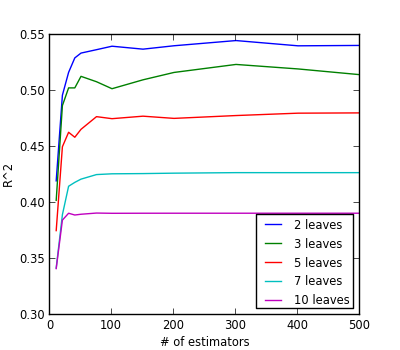
\includegraphics{test_r2s.png}
        \caption{$R^2$ of gradient boosting tree models on the test dataset as a function of the number of estimator iterations. The different curves represent different numbers of leaves in the weak learner decision trees. The simplest weak learner, a 2-leaf tree, performs the best. Using stochastic gradient boosting trees, in which a subsample of the features are used to fit the decision trees, improved the high-leaf models to some degree. This suggests that the inferior performance of the higher-leaf models may be due to overfitting.}
        \label{fig:gradient-params}
    \end{figure}
    
    \paragraph{}
    I tried a few different prediction algorithms; the one that proved the most effective on the test set, as measured by $R^2$, was gradient boosting trees.\footnote{Random forests and ordinary linear regression performed worse, but not by much. Despite the clearly non-normal distribution of the revenue per theater (it has a positive skew), I did not have better success with a generalized linear regression than with ordinary linear regression.} Gradient boosting is a general predictive technique pioneered by Jerome Friedman of Stanford in which a predictive formula is generated by summing so-called ``weak predictors'' that are sequentially fit to the gradient of a specified loss function (for example, squared error). The overall model may be accurate and robust even if each individual weak predictor is very simplistic. Gradient boosting trees refers to gradient boosting with decision trees as our weak predictors. For details, see Friedman's article \cite{bib:greedy-function}, and also Wikipedia's own page on gradient boosting \cite{bib:wikipedia-gradient-boosting}. 

    \paragraph{}
    I used the Python statistical package \textsf{scikit-learn}'s implementation of gradient boosting trees, using the default learning rate and least squares as my loss function. There are a few other model parameters that can be controlled in the user; the most important ones are the number of estimators (the number of weak predictors to fit) and the depth of the trees (how many leaves are in each decision tree - this parameterizes the complexity of each individual weak predictor). 
    
    \paragraph{}
    Adapting the example in \textsf{scikit-learn}'s documentation \cite{bib:scikit-ensemble}, I calculated the $R^2$ of gradient boosting trees at different iterations and tree depths. I fit the model at different parameterizations to the test data. Figure~\ref{fig:gradient-params} illustrates the results, and shows that this model fits the test data best with about 100 iterations (this is in fact \textsf{scikit-learn}'s default value) and a very simple 2-leaf functional form for its weak predictors. 
    
    \begin{figure}[ht]
        \centering
        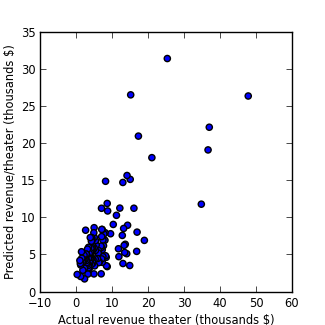
\includegraphics{pred_actual.png}
        \caption{Predicted values vs. actual values.}
        \label{fig:pred-actual}
    \end{figure}
    
    \paragraph{}
    Using a gradient boosting tree model with 100 estimators and 2 leaves in each weak learner, and training on films from 2007 to 2011 as mentioned previously, I was able to achieve an $R^2$ of 0.5400 on the 2012 dataset. The predictions and results are listed in an appendix at the end of this paper. Figure~\ref{fig:pred-actual} shows a scatter of predictions and actual values. 
    
    \paragraph{}
    The frequency with which a feature is used in the model's decision trees is representative of its importance in generating predictions; highly relevant features will be frequently involved in trees and irrelevant features will be involved rarely or not at all. Figure~\ref{fig:feature-importance} shows the top 10 features. Several features had frequencies of 0, in particular the boolean variables for several of the genre categories, indicating that they could have been completely omitted without impacting the outcomes of this model. 
    
    \begin{figure}[ht]
        \vspace{0.25in}
        \centering
        \footnotesize
        \begin{tabular}{l|r}
            Feature & Frequency (\%) \\
            \hline
            Wikipedia edit runs 7-28 days prior & 18.31 \\
            Film runtime & 14.60 \\
            Opening per theater revenue of similar films & 13.30 \\
            Wikipedia frequency of headers/subheaders & 12.07 \\
            Wikipedia edit runs 0-7 days prior & 10.97 \\
            Wikipedia average size of revisions & 9.73 \\
            Wikipedia frequency of word ``IMAX'' & 5.07 \\
            Wikipedia frequency of external files & 4.62 \\
            Is comedy & 3.74 \\
            MPAA rating is PG-13 & 3.17 
        \end{tabular}
        \caption{Top 10 features in the gradient boosting tree model.}
        \label{fig:feature-importance}
    \end{figure}
    
    \paragraph{}
    The importance of the Wikipedia data in this model can also be seen by removing the Wikipedia features and rerunning the model, which produces a considerable lower $R^2$ of 0.3434. 
    
    \section{Conclusion and avenues for further exploration}
    
    \paragraph{}
    While the results above do show that Wikipedia activity has some ability to predict box office returns, I do not think the model in this paper is precise enough to be used as anything but a very rough forecasting tool. Wikipedia is just one possible source of data for quantifying social interest; social networks such as Twitter or Facebook are another; frequency of appearance in news headlines is another.\footnote{In fact, I found that the number of opening theaters itself has significant predictive power on per-theater revenue. I omitted it mainly because I wanted to specifically examine Wikipedia's ability to measure social interest.} There are many conceivable metrics to gauge popular interest in seeing a film, and a comprehensive model would include data from many sources
    
    \paragraph{}
     In particular, a many-source approach will help overcome the biases that any one source would have. Although Wikipedia is widely known and read and edited by a wide variety of people, it will still be biased to whatever extent that Wikipedia editors do not reflect the population of people who go to the movies. It is my opinion that the best way to improve this model would be to obtain more measurements of popular interest, particularly data sources whose audiences overlap little with Wikipedia editors - measurements of interest among moviegoing demographics that use the Internet relatively infrequently, for example. 
    
    \paragraph{}
    Nevertheless, the partial success in predicting box office revenues with Wikipedia demonstrates that it is one potential source of data to consider when gauging interest - and not just in films, but anywhere popular interest is a concern. Wikipedia could be conceivably used as an input for predictions related to interest in news and current events, ticket sales for events other than films, investor sentiments, and many other areas. 
    
    \section{References and resources}
    
    \subsection{APIs and software packages}
    
    All data work was done in Python. The software packages that I used were: 
    
    \begin{itemize}
        \item \textsf{NumPy} (\url{http://www.numpy.org/}) - Popular package for doing general mathematical work. 
        \item \textsf{pandas} (\url{http://pandas.pydata.org/}) - Offers data structures and functions specific to statistical work. 
        \item \textsf{scikit-learn} (\url{http://scikit-learn.org/}) - Offers a variety of algorithms and useful functions for machine learning, prediction, error checking and validation, and so on. 
        \item \textsf{Beautiful Soup} (\url{http://www.crummy.com/software/BeautifulSoup/}) - Library to parse HTML. 
        \item \textsf{matplotlib} (\url{http://matplotlib.org/}) - Used to generate the graphics in this paper. 
        \item \textsf{simplejson} (\url{http://pypi.python.org/pypi/simplejson/}) - Used to parse the JSON-formatted data returned by the data sources' APIs. 
        \item \textsf{PyYAML} (\url{http://pyyaml.org/}) - A package to read YAML (Yet Another Markup Language, in my opinion a bit more flexible and human-editor-friendly than JSON). I formatted my scripts' configuration files in YAML. 
        \item \textsf{Joblib} (\url{http://packages.python.org/joblib/}) - I used this just for its pickling functionality, to save Wikipedia revision data locally so that I wouldn't have to requery the API repeatedly. 
    \end{itemize}
    
    Two of the data sources I used, Rotten Tomatoes and Wikipedia, offered APIs. Documentation on those can be found here: 
    
    \begin{itemize}
        \item Rotten Tomatoes API: \url{http://developer.rottentomatoes.com/}
        \item Wikipedia API: \url{http://en.wikipedia.org/w/api.php} - This is the documentation for MediaWiki-based websites that is returned when you query the API without any parameters
        \item MediaWiki API documentation: (\url{http://www.mediawiki.org/wiki/API:Main_page}) - Another handy resource, written more informally. 
    \end{itemize}
    
    \subsection{Bibliography}
    
    \begingroup
    \renewcommand{\section}[2]{}  % removes the header - thanks to http://tex.stackexchange.com/questions/22645/hiding-the-title-of-the-bibliography
    \begin{thebibliography}{1}
        
        \bibitem{bib:scikit-ensemble} ``Ensemble methods.'' Retrieved 13 Jan 2012. \url{http://scikit-learn.org/stable/modules/ensemble.html}
                
        \bibitem{bib:greedy-function} Friedman, Jerome H. (19 Apr 2001). ``Greedy Function Approximation: A Gradient Boosting Machine.'' Retrieved 10 Jan 2012. \url{http://www-stat.stanford.edu/~jhf/ftp/trebst.pdf}
        
        \bibitem{bib:wikipedia-gradient-boosting} ``Gradient boosting.'' Retrieved 13 Jan 2012. \url{http://en.wikipedia.org/wiki/Gradient_boosting}

        \bibitem{bib:wikipedia-hoaxes} ``List of hoaxes on Wikipedia.'' Retrieved 10 Jan 2012. \url{http://en.wikipedia.org/wiki/Wikipedia:List_of_hoaxes_on_Wikipedia}
        
        \bibitem{bib:bicholm} Pfeiffer, Eric (4 Jan 2013). ``War is over: Imaginary `Bicholm' conflict removed from Wikipedia after five years.'' Retrieved 10 Jan 2012. \url{http://news.yahoo.com/blogs/sideshow/war-over-imaginary-bicholim-conflict-page-removed-wikipedia-234717353.html}
        
        \bibitem{bib:wikipedia} ``Wikipedia.'' Retrieved 10 Jan 2012. \url{http://en.wikipedia.org/wiki/Wikipedia}
        
    \end{thebibliography}
    \endgroup
    
    \newpage
    
    \begin{figure}[ht]
        \scriptsize
        \centering
        \begin{tabular}{l|r|r|r}
            Title & Actual & Predicted & Error (actual - predicted) \\
            \hline
            Marvel's The Avengers & 47698 & 26452 & 21247 \\
            The Hunger Games & 36871 & 22247 & 14624 \\
            The Dark Knight Rises & 36532 & 19194 & 17338 \\
            The Twilight Saga: Breaking Dawn Part 2 & 34660 & 11890 & 22770 \\
            Skyfall & 25211 & 31496 & -6285 \\
            The Hobbit: An Unexpected Journey & 20919 & 18152 & 2767 \\
            Dr. Seuss' The Lorax & 18830 & 7018 & 11812 \\
            The Amazing Spider-Man & 17176 & 21054 & -3877 \\
            Ted & 16800 & 8127 & 8673 \\
            Think Like a Man & 16693 & 5536 & 11157 \\
            Brave & 15928 & 11344 & 4584 \\
            Prometheus & 15032 & 26608 & -11576 \\
            Snow White and the Huntsman & 14900 & 15231 & -331 \\
            The Devil Inside & 14763 & 3633 & 11129 \\
            Madagascar 3: Europe's Most Wanted & 14166 & 9051 & 5114 \\
            Les Miserables & 14015 & 15750 & -1735 \\
            The Vow & 13929 & 5224 & 8705 \\
            Taken 2 & 13525 & 6490 & 7035 \\
            Magic Mike & 13354 & 5383 & 7971 \\
            Flight & 13217 & 6345 & 6872 \\
            Wreck-It Ralph & 13070 & 8619 & 4451 \\
            Safe House & 12880 & 3902 & 8978 \\
            Men in Black 3 & 12851 & 14814 & -1962 \\
            Hotel Transylvania & 12697 & 7685 & 5012 \\
            Ice Age: Continental Drift & 12015 & 11360 & 654 \\
            Madea's Witness Protection & 11749 & 4824 & 6925 \\
            21 Jump Street & 11632 & 5887 & 5745 \\
            Django Unchained & 11070 & 10390 & 680 \\
            The Bourne Legacy & 10185 & 9162 & 1023 \\
            Wrath of the Titans & 9438 & 7910 & 1528 \\
            The Expendables 2 & 8622 & 10977 & -2355 \\
            Contraband & 8505 & 3486 & 5019 \\
            Paranormal Activity 4 & 8501 & 11988 & -3487 \\
            The Campaign & 8296 & 3597 & 4699 \\
            Underworld Awakening & 8222 & 4731 & 3491 \\
            Act of Valor & 8054 & 4942 & 3112 \\
            John Carter & 8050 & 14971 & -6920 \\
            Dark Shadows & 7906 & 8058 & -153 \\
            Journey 2: The Mysterious Island & 7878 & 7045 & 833 \\
            Chronicle & 7569 & 7876 & -306 \\
            Red Tails & 7477 & 6304 & 1173 \\
            The Woman in Black & 7311 & 7075 & 237 \\
            Tyler Perry's Good Deeds & 7310 & 4824 & 2485 \\
            The Lucky One & 7137 & 4066 & 3072 \\
            Sinister & 7126 & 5747 & 1380 \\
            Total Recall & 7103 & 8488 & -1385 \\
            Resident Evil: Retribution & 6989 & 8491 & -1501 \\
            Ghost Rider: Spirit of Vengeance & 6968 & 4521 & 2446 \\
            Looper & 6952 & 7526 & -573 \\
            Battleship & 6920 & 11337 & -4417 \\
            Project X & 6891 & 6061 & 830 \\
            Chimpanzee & 6829 & 2512 & 4317 \\
            American Reunion & 6740 & 6247 & 493 \\
            The Possession & 6297 & 4131 & 2166 \\
            The Grey & 6174 & 4020 & 2154 \\
            Savages & 6095 & 5649 & 445 \\
            Argo & 6020 & 5313 & 708 \\
            Life of Pi & 5805 & 4569 & 1236 \\
            This Means War & 5458 & 6400 & -942 \\
            \hline
        \end{tabular}
        \caption{2012 predictions and errors, sorted by actual revenue per theater}
    \end{figure}
    
    \begin{figure}[ht]
        \scriptsize
        \centering
        \begin{tabular}{l|r|r|r}
            Title & Actual & Predicted & Error (actual - predicted) \\
            \hline
            Abraham Lincoln: Vampire Hunter & 5247 & 5668 & -421 \\
            The Cabin in the Woods & 5245 & 6979 & -1734 \\
            Sparkle & 5189 & 4511 & 677 \\
            Mirror Mirror & 5032 & 3589 & 1444 \\
            Red Dawn & 4916 & 7430 & -2514 \\
            The Three Stooges & 4892 & 5981 & -1089 \\
            Rise of the Guardians & 4869 & 8725 & -3856 \\
            End of Watch & 4818 & 2503 & 2315 \\
            Cloud Atlas & 4787 & 8046 & -3259 \\
            Step Up Revolution & 4570 & 4409 & 162 \\
            Jack Reacher & 4538 & 5726 & -1188 \\
            Alex Cross & 4489 & 3955 & 533 \\
            That's My Boy & 4440 & 6258 & -1818 \\
            Parental Guidance & 4392 & 4140 & 252 \\
            Diary of a Wimpy Kid: Dog Days & 4312 & 5826 & -1514 \\
            The Dictator & 4245 & 7210 & -2965 \\
            The Secret World of Arrietty & 4235 & 6930 & -2695 \\
            The Man with the Iron Fists & 4235 & 6053 & -1818 \\
            One For the Money & 4207 & 4619 & -411 \\
            Rock of Ages & 4161 & 7405 & -3244 \\
            ParaNorman & 4108 & 6899 & -2791 \\
            Joyful Noise & 4104 & 3791 & 313 \\
            The Watch & 4025 & 5435 & -1411 \\
            House at the End of The Street & 3985 & 5928 & -1942 \\
            This Is 40 & 3976 & 5154 & -1178 \\
            Here Comes the Boom & 3921 & 4479 & -559 \\
            Hope Springs & 3850 & 5357 & -1507 \\
            Frankenweenie & 3798 & 7396 & -3599 \\
            Trouble with the Curve & 3786 & 4652 & -866 \\
            Big Miracle & 3645 & 4006 & -361 \\
            The Five-Year Engagement & 3614 & 4890 & -1276 \\
            What to Expect When You're Expecting & 3491 & 5260 & -1769 \\
            Safe & 3483 & 3176 & 307 \\
            Haywire & 3454 & 3687 & -232 \\
            The Pirates! Band of Misfits & 3317 & 6083 & -2766 \\
            The Raven & 3309 & 3317 & -8 \\
            Chernobyl Diaries & 3270 & 4665 & -1395 \\
            A Thousand Words & 3268 & 4619 & -1351 \\
            Wanderlust & 3260 & 3647 & -387 \\
            Silent House & 3136 & 2481 & 655 \\
            Katy Perry: Part of Me & 3031 & 5843 & -2812 \\
            The Odd Life of Timothy Green & 2954 & 3826 & -872 \\
            Seven Psychopaths & 2821 & 4024 & -1203 \\
            Killing Them Softly & 2811 & 5026 & -2215 \\
            Silent Hill: Revelation 3D & 2735 & 5153 & -2417 \\
            Lockout & 2700 & 4342 & -1642 \\
            Premium Rush & 2674 & 4297 & -1623 \\
            Man on a Ledge & 2669 & 5169 & -2500 \\
            Dredd & 2505 & 8384 & -5879 \\
            Seeking a Friend for the End of the World & 2352 & 4462 & -2109 \\
            The Collection & 2213 & 1832 & 381 \\
            Gone & 2182 & 3289 & -1106 \\
            People Like Us & 2071 & 5024 & -2953 \\
            Playing for Keeps & 2027 & 4417 & -2390 \\
            Atlas Shrugged: Part II & 1731 & 2991 & -1260 \\
            Lawless & 1700 & 4400 & -2701 \\
            The Words & 1696 & 4066 & -2370 \\
            The Guilt Trip & 1448 & 4619 & -3171 \\
            Fun Size & 1361 & 5487 & -4127 \\
            The Cold Light of Day & 1212 & 3987 & -2775 \\
            Chasing Mavericks & 1133 & 3702 & -2569 \\
            Last Ounce of Courage & 1127 & 2156 & -1029 \\
            Won't Back Down & 1035 & 3902 & -2867 \\
            Hit and Run & 910 & 4311 & -3401 \\
            Oogieloves In The BIG Balloon Adventure & 162 & 2429 & -2267 \\
            \hline
        \end{tabular}
        \caption{2012 predictions and errors (continued), sorted by actual revenue per theater}
    \end{figure}
    
\end{document}